%
%  $Description: Author guidelines and sample document in LaTeX 2.09$ 
%
%  $Author: John Burchell & William Granli $
%  $Date: 2015/01/21 15:20:59 $
%  $Revision: 1.0
%

\documentclass[10pt,twocolumn]{article} 
\usepackage{latex8}
\usepackage{url}
\usepackage{verbatim}
\usepackage{fixltx2e}
\usepackage{graphicx}
\usepackage{enumitem}
%\documentstyle[times,art10,twocolumn,latex8]{article}

%------------------------------------------------------------------------- 
% take the % away on next line to produce the final camera-ready version 
\pagestyle{empty}

%------------------------------------------------------------------------- 
\begin{document}



\title{Assignment 4}

% author names and affiliations
\author{John Burchell and William Granli \\
john.a.burchell, william.granli@gmail.com}


\maketitle
\thispagestyle{empty}

%------------------------------------------------------------------------- 

\section{Introduction}
Software inspections have since its inception [1] more than
25 years ago spawned quite some interest both from the
research community and industrial practice. The research
includes changes to the inspection process, e.g. [2], support to
the proceThe dependent variables are analyzed to evaluate the
hypotheses of the experiment. The main null and alternative
hypotheses [12] are stated below. These are evaluated for all
faults, class A faults and class A\&B faults. The hypotheses
concern efficiency, effectiveness and fault detecting
differences:ss, e.g. [3] and empirical studies, e.g. [4]. The
suggested improvements include active design reviews [5] and
perspective-based reading [6]. Industry has studied the
benefits of conducting software inspections [7].

\section{Purpose of the Study}
This section will describe the purpose of the study, the research questions and the hypotheses. 

\subsection{Purpose Statement}
The objective of this study is to compare and hence
evaluate how well the use-case based reading performs in
comparison to other methods. The study presents a controlled
experiment where use-case based reading is compared to
checklist-based reading.

\subsubsection{Variables}
Three types of variables are defined for the experiment,
independent, controlled, and dependent variables.

\begin{enumerate}[label=(\alph*)]

\item Independent Variable: The independent variable is
the reading technique used. The experiment groups used either
Use-Cased Based Reading or Checklist-Based Reding.
\item Controlled Variable: The controll variable is the
experience of the reviwers and it is measured on an ordinal
scale. The reviwers were asked to fill in a questionnare
comprising seven questions.
\item Dependent Variables: The dependent varialbles
measured are faults. The four variables are: (1) Number of
faults found by each reviwer, (2) Number of faults found by
each experiment group, (3) efficiency (faults/hour) and is
measured as: 60*(number of fault found/inspection time which
is 45 min), and (4) effectivness (detection rate) and is mesured
as: number of faults found/total number of faults.

\end{enumerate}

\subsection{Research Questions}

\subsection{Hypothesis}
The general hypothesis of the experiment is that Use-Case
Based Reading is more efficient and effective in finding faults
of the most critical fault classes, i.e. Checklist-Based Reading
is assumed to find more faults per time unit, and to find a
larger rate of the critical faults.
The dependent variables are analyzed to evaluate the
hypotheses of the experiment. The main null and alternative
hypotheses [12] are stated below. These are evaluated for all
faults, class A faults and class A\&B faults. The hypotheses
concern efficiency, effectiveness and fault detecting
differences:
\begin{itemize}
\item H\textsubscript{0 Eff} - There is no difference in efficiency (i.e.found faults per hour) between the reviewers applying use cases and the reviewers using a checklist.
\item H\textsubscript{1 Eff} - There is a difference in efficiency between the reviewers applying prioritized use cases and the reviewers using a checklist.
\item H\textsubscript{0 Rate} - There is no difference in effectiveness (i.e. rate of faults found) between the reviewers applying use cases and the reviewers using a checklist.
\item H\textsubscript{1 Rate} - There is a difference in effectiveness between the reviewers applying use cases and the reviewers using a checklist.
\item H\textsubscript{0 Fault} - The reviewers applying use cases do not detect different faults than the reviewers using a checklist.
\item H\textsubscript{1 Fault} - The reviewers applying use cases detect different faults than the reviewers using a checklist.

\end{itemize}

\Section{Methodology}
This section will describe which statistical tests were used, and why. The level of significance used for all tests is 0.05. 

\SubSection{Tests Used for H\textsubscript{eff} and H\textsubscript{rate}}
Initially, Kolmogorov-Smirnov (KS) Goodness-of-Fit and Shapiro-Wilks (SW) tests were used to determine if the assumption of normality could be held for the data set. The data used for the tests was the number faults found by each participant. The reason this data was chosen was that it directly correlates to the data used in H\textsubscript{eff} and H\textsubscript{rate}. The KS and SW tests both reported p-values < 0.05. See Table 1 for the p-values of the KS and SW tests. The critical value analysis for the KS and SW showed similar results and thus the null hypotheses of the data being normally distributed was rejected. See Table 2 for more information about the critical value results of the KS and SW tests.

\begin{table}
	\centering
	\begin{tabular}[ht]{| l | l | l |}
	\hline
	Test & Sample & p-value  \\
	\hline
	KS & UC & \textless 2.2e-16 \\
	\hline
	SW & UC & 0.000969 \\
	\hline
	KS & CL & \textless 2.2e-16 \\
	\hline
	SW & CL & 0.309 \\	
	\hline
	\end{tabular}
	\caption{KS \& SW tests - p-value}
\end{table}


\begin{table}
	\centering
	\begin{tabular}[ht]{| l | l | l | l |}
	\hline
	Test & Sample & Critical Value & D (result)  \\
	\hline
	KS & UC & 0.270 & 0.9388 \\
	\hline
	SW & UC & 0.964 &  0.8412 \\
	\hline
	KS & CL & 0.270 & 0.9388 \\
	\hline
	SW & CL & 0.964 & 0.9553 \\	
	\hline
	\end{tabular}
	\caption{KS \& SW tests - Critical Value}
\end{table}


A graphical representation of the level of normalisation can be seen in Figure 1 and 2. The results from the tests are supported by the sparseness of the data points. 

\begin{figure}[ht]
\centering
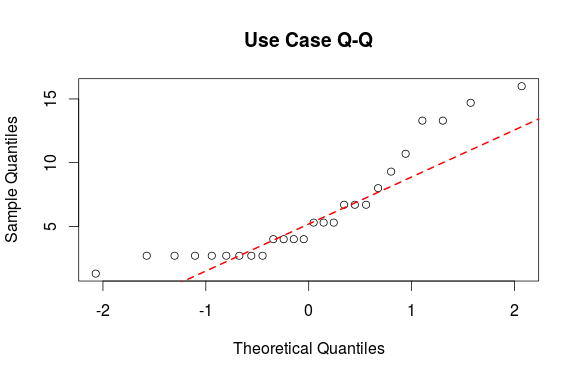
\includegraphics[width=90mm]{uc_qq.png}
\caption{Use Case Q-Q plot}
\end{figure}

\begin{figure}[ht]
\centering
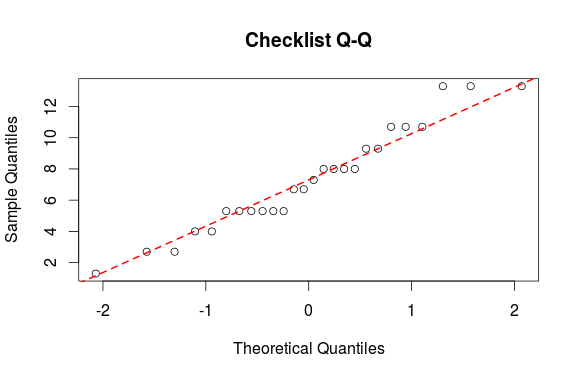
\includegraphics[width=90mm]{cl_qq.png}
\caption{Checklist Q-Q plot}
\end{figure}


The next step was to perform an outlier test. The method used was boxplots. As seen in Figure 3 and 4, no outliers were detected and thus no data points were removed in the tests performed. 

\begin{figure}[ht]
\centering
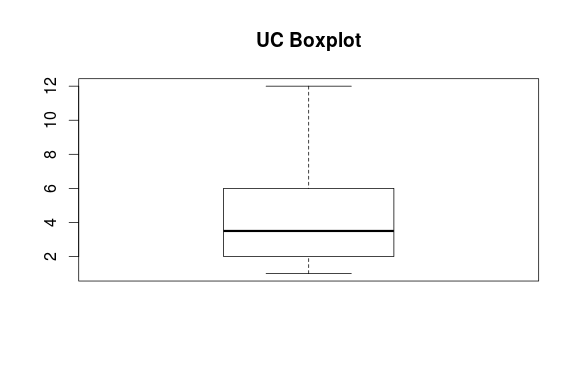
\includegraphics[width=90mm]{uc_box.png}
\caption{Use Case Boxplot}
\end{figure}

\begin{figure}[ht]
\centering
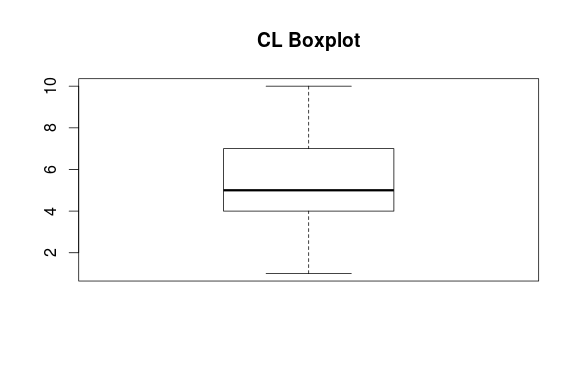
\includegraphics[width=90mm]{cl_box.png}
\caption{Checklist Boxplot}
\end{figure}


\Section{Results}

\subsection{There is no difference in efficiency}
Since the data is non-normalised, the Wilcoxon-Mann-Whitney (WMW) two-sample rank-sum test was chosen instead of the Student's T-test as the final test. The data used for the WMW test was the efficiency of each participant. The result of the WMW test was W=250, p=0.1063 and with the significance level of 536, thus the null hypothesis H\textsubscript{0} Eff is rejected. 

\subsection{There is no difference in effectiveness}
The same test was chosen for Hrate, based on the same reasoning. The result of the WMW test for Hrate was W=250, p=0.1063 and with the significance level of 536 thus the null hypothesis H\textsubscript{0} Rate is rejected. 


\subsection{Results for Hfault}

data:  data.table
X-squared = 1.5998, df = 2, p-value = 0.4494

http://www.sussex.ac.uk/Users/grahamh/RM1web/WilcoxonTable2005.pdf



MWW = good for cont tests as well.
 Mann, Henry B.; Whitney, Donald R. (1947). ``On a Test of Whether one of Two Random Variables is Stochastically Larger than the Other''. Annals of Mathematical Statistics 18 (1): 50–60. doi:10.1214/aoms/1177730491. MR 22058. Zbl 0041.26103.







\Section{Tests for eff}


\Section{Tests for 3}



Chi-square test requirements[edit]
Quantitative data.
One or more categories.
Independent observations.
Adequate sample size (at least 10).
Simple random sample.
Data in frequency form.
All observations must be used.
\bibliographystyle{latex8}
\bibliography{latex8}


\Section{Acknowledgements}
U w0T m8


\end{document}

